\documentclass[12pt,fleqn]{article}
\usepackage{vkCourseML}
\hypersetup{unicode=true}
%\usepackage[a4paper]{geometry}
\usepackage[hyphenbreaks]{breakurl}

\interfootnotelinepenalty=10000

\begin{document}
\title{Лекция 2\\Линейная регрессия}
\author{Е.\,А.\,Соколов\\ФКН ВШЭ}
\maketitle

\section{Линейные модели}

На предыдущей лекции мы уже упоминали линейные регрессионные модели.
Такие модели сводятся к суммированию значений признаков с некоторыми весами:

\begin{equation}
\label{eq:linear}
    a(x)
    =
    w_0
    +
    \sum_{j = 1}^{d}
        w_j x_j.
\end{equation}
Параметрами модели являются~\emph{веса} или~\emph{коэффициенты}~$w_j$.
Вес~$w_0$ также называется свободным коэффициентом или \emph{сдвигом}~(bias).
Заметим, что сумма в формуле~\eqref{eq:linear} является скалярным произведением
вектора признаков на вектор весов.
Воспользуемся этим и запишем линейную модель в более компактном виде:
\begin{equation}
\label{eq:linearCompact}
    a(x)
    =
    w_0
    +
    \langle w, x \rangle,
\end{equation}
где~$w = (w_1, \dots, w_d)$~--- вектор весов.

Достаточно часто используется следующий приём, позволяющий упростить запись ещё сильнее.
Добавим к признаковому описанию каждого объекта $(d + 1)$-й признак, равный единице.
Вес при этом признаке как раз будет иметь смысл свободного коэффициента,
и необходимость в слагаемом~$w_0$ отпадёт:
\[
    a(x)
    =
    \langle w, x \rangle.
\]
Тем не менее, при такой форме следует соблюдать осторожность и помнить
о наличии в выборке специального признака.
Например, мы столкнёмся со сложностями, связанными с этим, когда будем говорить о регуляризации.

За счёт простой формы линейные модели достаточно быстро и легко обучаются,
и поэтому популярны при работе с большими объёмами данных.
Также у них мало параметров, благодаря чему удаётся контролировать риск переобучения
и использовать их для работы с зашумлёнными данными и с небольшими выборками.

\section{Области применимости линейных моделей}

Сложно представить себе ситуацию, в которой мы берём данные, обучаем линейную модель и получаем хорошее качество работы.
В линейной модели предполагается конкретный вид зависимости~--- а именно, что каждый признак линейно влияет на целевую переменную,
и что целевая переменная не зависит от каких-либо комбинаций признаков.
Вряд ли это будет выполнено по умолчанию, поэтому обычно данные требуют специальной подготовки, чтобы линейные модели
оказались адекватными задаче.
Приведём несколько примеров.

\paragraph{Категориальные признаки.}
Представим себе задачу определения стоимости квартиры по её характеристикам.
Одним из важных признаков является район, в котором находится квартира.
Этот признак является категориальным~--- его значения нельзя сравнивать между собой на больше/меньше,
их нельзя складывать или вычитать.
Непосредственно такие признаки нельзя использовать в линейных моделях, но есть
достаточно распространённый способ их преобразования.

Допустим, категориальный признак~$f_j(x)$ принимает значения из множества~$C = \{c_1, \dots, c_m\}$.
Заменим его на~$m$ бинарных признаков~$b_1(x), \dots, b_m(x)$, каждый из которых
является индикатором одного из возможных категориальных значений:
\[
    b_i(x) = [f_j(x) = c_i].
\]
Такой подход называется one-hot кодированием.

Отметим, что признаки~$b_1(x), \dots, b_m(x)$ являются линейно зависимыми:
для любого объекта выполнено
\[
    b_1(x) + \dots + b_m(x) = 1.
\]
Чтобы избежать этого, можно выбрасывать один из бинарных признаков.
Впрочем, такое решение имеет и недостатки~--- например, если на тестовой выборке
появится новая категория, то её как раз можно закодировать с помощью нулевых бинарных признаков;
при удалении одного из них это потеряет смысл.

Вернёмся к задаче про стоимость квартиры.
Если мы применим линейную модель к данным после one-hot кодирования признака о районе~(допустим, это $f(x)$), то получится
такая формула:
\[
    a(x)
    =
    w_1 [f(x) = c_1]
    +
    \dots
    +
    w_m [f(x) = c_m]
    +
    \{
        \text{взаимодействие с другими признаками}
    \}.
\]
Такая зависимость кажется логичной~--- каждый район задаёт некоторый базовый уровень
стоимости~(например, для района~$c_1$ имеем базовую цену~$w_1$),
а остальные факторы корректируют его.

\paragraph{Работа с текстами.}

Перейдём к предсказанию стоимости квартиры по её текстовому описанию.
Есть простой способ кодирования, который называется~\emph{мешок слов~(bag of words)}.

Найдём все слова, которые есть в нашей выборке текстов, и пронумеруем их:~$\{c_1, \dots, c_m\}$.
Будем кодировать текст~$m$ признаками~$b_1(x), \dots, b_m(x)$, где~$b_j(x)$ равен
количеству вхождений слова~$c_j$ в текст.
Линейная модель над такими признаками будет иметь вид
\[
    a(x)
    =
    w_1 b_1(x)
    +
    \dots
    +
    w_m b_m(x)
    +
    \dots,
\]
и такой вид тоже кажется разумным.
Каждое вхождение слова~$c_j$ меняет прогноз стоимости на~$w_j$.
В самом деле, можно ожидать, что слово~<<престижный>> скорее говорит о том,
что квартира дорогая, а слово~<<плохой>> вряд ли будут использовать при описании
приличной квартиры.

\paragraph{Бинаризация числовых признаков.}

Наконец, подумаем о предсказании стоимости квартиры по расстоянию до ближайшей станции метро~$x_j$.
Может оказаться, что самые дорогие квартиры расположены где-то в 5-10 минутах ходьбы от метро,
а те, что ближе или дальше, стоят не так дорого.
В этом случае зависимость целевой переменной от признака не будет линейной.
Чтобы сделать линейную модель подходящей, мы можем бинаризовать признак.
Для этого выберем некоторую сетку точек~$\{t_1, \dots, t_m\}$.
Это может быть равномерная сетка между минимальным и максимальным значением признака или,
например, сетка из эмпирических квантилей.
Добавим сюда точки~$t_0 = -\infty$ и~$t_{m+1} = +\infty$.
Новые признаки зададим как
\[
    b_i(x)
    =
    [t_{i - 1} < x_j \leq t_{i}],
    \quad
    i = 1, \dots, m+1.
\]
Линейная модель над этими признаками будет выглядеть как
\[
    a(x)
    =
    w_1 [t_{0} < x_j \leq t_{1}]
    +
    \dots
    +
    w_{m+1} [t_{m} < x_j \leq t_{m+1}]
    +
    \dots,
\]
то есть мы найдём свой прогноз стоимости квартиры для каждого интервала расстояния до метро.
Такой подход позволит учесть нелинейную зависимость между признаком и целевой переменной.

\section{Измерение ошибки в задачах регрессии}

Чтобы обучать регрессионные модели, нужно определиться, как именно измеряется качество предсказаний.
Будем обозначать через~$y$ значение целевой переменной, через~$a$~--- прогноз модели.
Рассмотрим несколько способов оценить отклонение~$L(y, a)$ прогноза от истинного ответа.

\paragraph{MSE и $R^2$.}

Основной способ измерить отклонение~--- посчитать квадрат разности:
\[
    L(y, a) = (a - y)^2
\]
Благодаря своей дифференцируемости эта функция наиболее часто используется в задачах регрессии.
Основанный на ней функционал называется среднеквадратичным отклонением~(mean squared error, MSE):
\[
    \text{MSE}(a, X)
    =
    \frac{1}{\ell}
    \sum_{i = 1}^{\ell} \left(
        a(x_i) - y_i
    \right)^2.
\]
Отметим, что величина среднеквадратичного отклонения плохо интерпретируется,
поскольку не сохраняет единицы измерения~--- так, если мы предсказываем цену
в рублях, то MSE будет измеряться в квадратах рублей.
Чтобы избежать этого, используют корень из среднеквадратичной ошибки~(root mean squared error, RMSE):
\[
    \text{RMSE}(a, X)
    =
    \sqrt{
        \frac{1}{\ell}
        \sum_{i = 1}^{\ell} \left(
            a(x_i) - y_i
        \right)^2
    }.
\]

Среднеквадратичная ошибка подходит для сравнения двух моделей
или для контроля качества во время обучения,
но не позволяет сделать выводы о том, насколько хорошо данная модель
решает задачу.
Например, $\text{MSE}=10$ является очень плохим показателем,
если целевая переменная принимает значения от 0 до 1,
и очень хорошим, если целевая переменная лежит в интервале~$(10000, 100000)$.
В таких ситуациях вместо среднеквадратичной ошибки полезно использовать~\emph{коэффициент детерминации}
(или коэффициент~$R^2$):
\[
    R^2(a, X)
    =
    1
    -
    \frac{
        \sum_{i = 1}^{\ell} (a(x_i) - y_i)^2
    }{
        \sum_{i = 1}^{\ell} (y_i - \bar y)^2
    },
\]
где~$\bar y = \frac{1}{\ell} \sum_{i = 1}^{\ell} y_i$~--- среднее значение целевой переменной.
Коэффициент детерминации измеряет долю дисперсии, объяснённую моделью, в общей дисперсии
целевой переменной.
Фактически, данная мера качества~--- это нормированная среднеквадратичная ошибка.
Если она близка к единице, то модель хорошо объясняет данные,
если же она близка к нулю, то прогнозы сопоставимы по качеству с константным предсказанием.

\paragraph{MAE.}

Заменим квадрат отклонения на модуль:
\[
    L(y, a) = |a - y|
\]
Соответствующий функционал называется средним абсолютным отклонением~(mean absolute error, MAE):
\[
    \text{MAE}(a, X)
    =
    \frac{1}{\ell}
    \sum_{i = 1}^{\ell} \left|
        a(x_i) - y_i
    \right|.
\]

Модуль отклонения не является дифференцируемым, но при этом менее чувствителен к выбросам.
Квадрат отклонения, по сути, делает особый акцент на объектах с сильной ошибкой,
и метод обучения будет в первую очередь стараться уменьшить отклонения на таких объектах.
Если же эти объекты являются выбросами~(то есть значение целевой переменной на них либо ошибочно,
либо относится к другому распределению и должно быть проигнорировано),
то такая расстановка акцентов приведёт к плохому качеству модели.
Модуль отклонения в этом смысле гораздо более терпим к сильным ошибкам.

\begin{table}[t]
\centering
\begin{tabular}[t]{|c||c|c|c||c|c|c|}
    \hline
    $y$ & $a_1(x)$ & $(a_1(x) - y)^2$ & $|a_1(x) - y|$ & $a_2(x)$ & $(a_2(x) - y)^2$ & $|a_2(x) - y|$  \\
    \hline
    1 & 2 & 1 & 1 & 4 & 9 & 3 \\
    2 & 1 & 1 & 1 & 5 & 9 & 3 \\
    3 & 2 & 1 & 1 & 6 & 9 & 3 \\
    4 & 5 & 1 & 1 & 7 & 9 & 3 \\
    5 & 6 & 1 & 1 & 8 & 9 & 3 \\
    {\color{red} 100} & 7 & 8649 & 93 & 10 & 8100 & 90 \\
    7 & 6 & 1 & 1 & 10 & 9 & 3 \\ \hline
      &   & $\text{MSE} = 1236$ & $\text{MAE} = 14.14$ & & $\text{MSE} = 1164$ & $\text{MAE} = 15.43$ \\
    \hline
\end{tabular}
\caption{Поведение MSE и MAE при наличии выбросов.}
\label{tab:outlier}
\end{table}

Рассмотрим для примера данные из таблицы~\ref{tab:outlier}.
Один из объектов~--- выброс, значение целевой переменной на нём радикально отличается
от остальных объектов.
Модель~$a_1(x)$ почти не ошибается на~<<нормальных>> объектах,
но сильно ошибается на выбросе.
Модель~$a_2(x)$ подгоняется под выброс ценой ухудшения прогнозов на остальных объектах.
Видно, что первая модель оказывается лучше с точки зрения MAE, но хуже с точки зрения MSE.
Это логично~--- у квадратичной функции потерь штраф за ошибку растёт нелинейно с ростом отклонения прогноза от ответа,
а для абсолютной функции потерь равносильно снижение отклонения на одну и ту же величину для нормального объекта и для выброса.
Заметим, что такая особенность MAE пропадёт, если в выборке будет много выбросов.
Скажем, если будет около половины объектов с аномальными значениями целевой переменной, то вполне
может стать выгоднее оптимизировать отклонение именно на них.

Приведём ещё одно объяснение того, почему модуль отклонения устойчив к выбросам,
на простом примере.
Допустим, все~$\ell$ объектов выборки имеют одинаковые признаковые описания, но разные
значения целевой переменной~$y_1, \dots, y_\ell$.
В этом случае модель должна на всех этих объектах выдать один и тот же ответ.
Если мы выбрали MSE в качестве функционала ошибки, то получаем следующую задачу:
\[
    \frac{1}{\ell}
    \sum_{i = 1}^{\ell} \left(
        a - y_i
    \right)^2
    \to
    \min_a
\]
Легко показать, что минимум достигается на среднем значении всех ответов:
\[
    a_{\text{MSE}}^*
    =
    \frac{1}{\ell}
    \sum_{i = 1}^{\ell}
        y_i.
\]
Если один из ответов на порядки отличается от всех остальных~(то есть является выбросом),
то среднее будет существенно отклоняться в его сторону.

Рассмотрим теперь ту же ситуацию, но с функционалом MAE:
\[
    \frac{1}{\ell}
    \sum_{i = 1}^{\ell} \left|
        a - y_i
    \right|
    \to
    \min_a
\]
Теперь решением будет медиана ответов:
\[
    a_{\text{MAE}}^*
    =
    \text{median}
        \{y_i\}_{i = 1}^{\ell}.
\]
Небольшое количество выбросов никак не повлияет на медиану~--- она существенно
более устойчива к величинам, выбивающимся из общего распределения.

В заключение отметим одну проблему, связанную с абсолютной функцией потерь.
Рассмотрим производные для неё и квадратичной функции:
\begin{align*}
    &\frac{\partial}{\partial a} |a - y| = \sign (a - y), \quad a \neq y; \\
    &\frac{\partial}{\partial a} (a - y)^2 = 2 (a - y).
\end{align*}
Дальше в курсе мы будем изучать градиентные методы обучения,
где параметры модели постепенно изменяются на основе значений производных функции потерь.
Видно, что производная абсолютной функции потерь не зависит от близости прогноза к правильному ответу,
по её значению нельзя понять, насколько мы близки к оптимальному прогнозу.
Из-за этого при оптимизации MAE можно легко~<<перескочить>> экстремум.
Поэтому, как правило, использование этой функции потерь приводит к более долгой и сложной
процедуре обучения.

\begin{figure}[t]
    \centering
    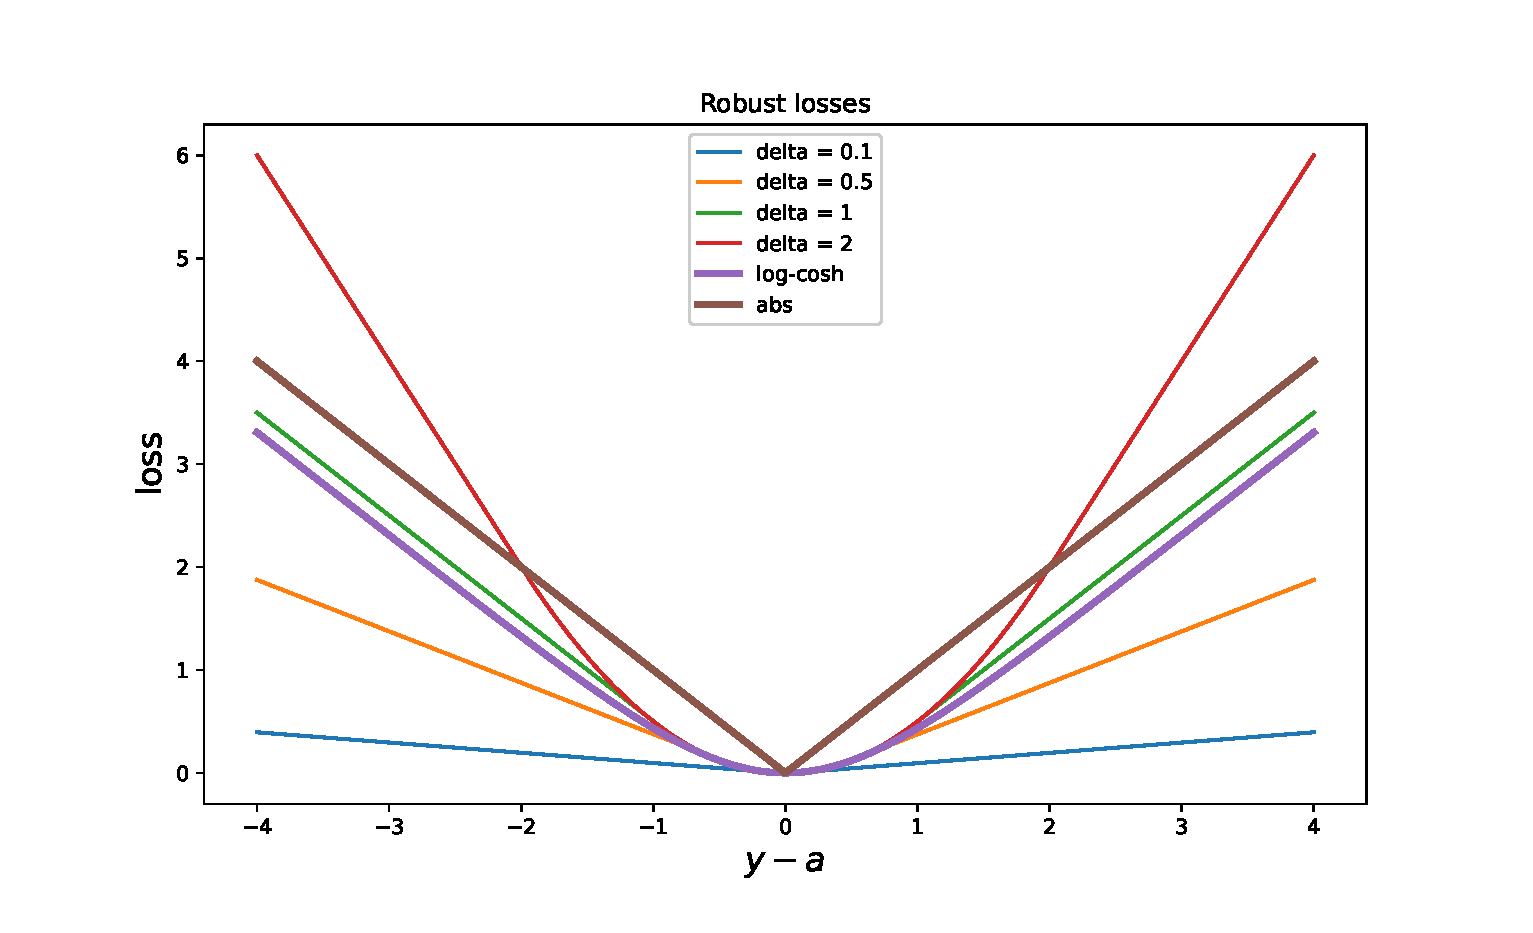
\includegraphics[width=1.0\textwidth]{pics/robust_losses.eps}
    \caption{Функция потерь Хубера и Log-Cosh.}
    \label{fig:robust_losses}
\end{figure}

\paragraph{Huber loss.}

Выше мы обсудили, что абсолютная функция потерь более устойчива к выбросам,
а квадратичная функция лучше с точки зрения оптимизации.
Почему бы не попробовать их объединить?
Для прогнозов, близких к ответу, нам бы пригодились свойства гладкой квадратичной функции,
а для плохих прогнозов важнее свойства абсолютного отклонения.
Одним из вариантов такого объединения является функция потерь Хубера:
\[
    L_\delta(y, a)
    =
    \left\{
    \begin{aligned}
        &\frac12 (y - a)^2, \quad |y - a| < \delta \\
        &\delta \left(
            |y - a| - \frac12 \delta
        \right), \quad |y - a| \geq \delta
    \end{aligned}
    \right.
\]

У этой функции потерь есть параметр~$\delta$, который регулирует, что мы считаем за выбросы.
Если сделать этот параметр маленьким, то функция будет вести себя квадратично только в маленькой окрестности нуля.
Если же увеличивать~$\delta$, то даже для значительных отклонений~$(a - y)$ штраф будет вести себя квадратично,
и при обучении мы будем делать большой акцент на их уменьшение.
Данный параметр надо подбирать, поскольку он может сильно повлиять на решение.

Также легко, что при~$\delta \to 0$ функция потерь Хубера вырождается в абсолютную функцию потерь,
а при~$\delta \to \infty$~--- в квадратичную.

\paragraph{Log-Cosh}

У функции потерь Хубера есть недостаток: её вторая производная имеет разрывы.
Такого недостатка нет у функции потерь log-cosh:
\[
    L(y, a)
    =
    \log \cosh(a - y).
\]

Как и в случае с функцией потерь Хубера, для маленьких отклонений здесь имеет место
квадратичное поведение, а для больших~--- линейное.

Обсужденные нами~<<гибридные>> функции потерь изображены на рис.~\ref{fig:robust_losses}.
Отметим, что существуют достаточно широкие обобщения этих функций потерь~\cite{barron19robust}.

\paragraph{MSLE.}

Перейдём теперь к логарифмам ответов и прогнозов:
\[
    L(y, a) = (\log(a + 1) - \log(y + 1))^2
\]
Соответствующий функционал называется среднеквадратичной логарифмической ошибкой~(mean
squared logarithmic error, MSLE).
Данная метрика подходит для задач с неотрицательной целевой переменной и неотрицательными прогнозами модели.
За счёт логарифмирования ответов и прогнозов мы скорее штрафуем за отклонения
в порядке величин, чем за отклонения в их значениях.
Также следует помнить, что логарифм не является симметричной функцией,
и поэтому данная функция потерь штрафует заниженные прогнозы сильнее,
чем завышенные.

\paragraph{MAPE и SMAPE.}

В задачах прогнозирования нередко измеряется относительная ошибка.
Во-первых, это удобно для интерпретации~--- легко понять, что~<<ошибка 50\%>>
соответствует отклонению в полтора раза от целевой переменной.
Во-вторых, это позволяет работать с разными мастштабами.
Например, мы можем решать задачу прогнозирования спроса на товары в магазине,
и какие-то товары могут продаваться штуками, а какие-то~--- тысячами.
Чтобы при усреднении ошибок более популярные товары не оказывали
большее влияние на результат, следует использовать функции потерь, не зависящие от масштаба.
Типичный пример относительной функции потерь:
\[
    L(y, a) = \left| \frac{y - a}{y} \right|
\]
Соответствующий функционал называется средней абсолютной процентной ошибкой~(mean
absolute percentage error, MAPE).

У MAPE есть проблем с несимметричностью: скажем, если~$y = 1$ и все прогнозы неотрицательные,
то максимальная ошибка при занижении прогноза~($a < y$) равна единице, а ошибка при
завышении прогноза~($a > y$) никак не ограничена сверху.
Это исправляется в симметричной модификации~(symmetric mean absolute percentage error, SMAPE):
\[
    L(y, a) = \frac{|y - a|}{(|y| + |a|) / 2}
\]

\paragraph{Квантильная функция потерь.}

В некоторых задачах цены занижения и завышения прогнозов могут отличаться друг от друга.
Например, при прогнозировании спроса на товары интернет-магазина гораздо опаснее заниженные
предсказания, поскольку они могут привести к потере клиентов.
Завышенные же прогнозы приводят лишь к издержкам на хранение товара на складе.
Функционал в этом случае можно записать как
\[
    Q(a, X^\ell)
    =
    \sum_{i = 1}^{\ell}
        \rho_\tau(y_i - a(x_i)),
\]
где
\[
    \rho_\tau(z)
    =
    (\tau - 1) [z < 0] z
    +
    \tau [z \geq 0] z
    =
    (\tau - \frac{1}{2})z + \frac{1}{2} |z|,
\]
а параметр~$\tau$ лежит на отрезке~$[0, 1]$ и определяет
соотношение важности занижения и завышения прогноза.
Чем больше здесь~$\tau$, тем выше штраф за занижение прогноза.

Обсудим вероятностный смысл данного функционала.
Будем считать, что в каждой точке~$x \in \XX$ пространства объектов
задано вероятностное распределение~$p(y \cond x)$ на возможных ответах для данного объекта.
Такое распределение может возникать, например, в задаче предсказания кликов по рекламным баннерам:
один и тот же пользователь может много раз заходить на один и тот же сайт и видеть данный баннер;
при этом некоторые посещения закончатся кликом, а некоторые~--- нет.

Известно, что при оптимизации квадратичного функционала алгоритм~$a(x)$
будет приближать условное матожидание ответа в каждой точке пространства
объектов:~$a(x) \approx \EE [y \cond x]$;
если же оптимизировать среднее абсолютное отклонение, то итоговый алгоритм
будет приближать медиану распределения:~$a(x) \approx \text{median} [p(y \cond x)]$.
Рассмотрим теперь некоторый объект~$x$ и условное распределение~$p(y \cond x)$.
Найдем  число~$q$, которое будет оптимальным с точки зрения нашего функционала:
\[
    Q = \int_\YY \rho_\tau(y - q) p(y \cond x) dy.
\]
Продифференцируем его~(при этом необходимо воспользоваться правилами
дифференцирования интегралов, зависящих от параметра):
\[
    \frac{\partial Q}{\partial q}
    =
    (1 - \tau) \int_{-\infty}^{q} p(y \cond x) dy
    -
    \tau \int_{q}^{\infty} p(y \cond x) dy
    =
    0.
\]
Получаем, что
\[
    \frac{\tau}{1 - \tau}
    =
    \frac{
        \int_{-\infty}^{q} p(y \cond x) dy
    }{
        \int_{q}^{\infty} p(y \cond x) dy
    }.
\]
Данное уравнение будет верно, если~$q$ будет равно~$\tau$-квантили распределения~$p(y \cond x)$.
Таким образом, использование функции потерь~$\rho_\tau(z)$ приводит к тому,
что алгоритм~$a(x)$ будет приближать~$\tau$-квантиль распределения ответов в каждой точке
пространства объектов.


\begin{thebibliography}{1}
\bibitem{barron19robust}
    \emph{Jonathan T. Barron} (2019).
    A General and Adaptive Robust Loss Function.~//
    \url{https://arxiv.org/pdf/1701.03077.pdf}.
\end{thebibliography}

\end{document}
